\subsection{开发语言}
Kubernetes生态的主流语言是Go,
在Serverless平台的开发中,
关于开发语言的资料相对较少,
但根据现有资料,
可以了解和推测:

\begin{itemize}
    \item 基于Kubernetes、Knative等Kubernetes生态的系统以Go为主;
    包括EasyFaaS、firecracker-containerd等也是使用Go开发
    \item 美团在建设Nest平台时没有选择Go而选择了Java作为主要语言,
    原因是因为美团内部Java占主导地位\cite{meituan_serverless_nest};
    另外Apache OpenWhisk主要是Scala实现
    \item Rust有较多的应用,例如Firecracker使用Rust开发,字节使用了Rust/WebAssembly\cite{bytedance_faas}
\end{itemize}


\subsection{Serverless平台架构设计}
\subsubsection{调用模式和方式}
典型的Serverless架构是基于事件驱动的模式,
根据调用模型又可以分为同步模式和异步模式两种。
同步模式下,
客户端调用后等待函数运行完成得到结果;
异步模式下,
客户端触发调用后即完成,
通常采用事件队列的方式来实现异步调用\cite{aws_lambda_2022}。

Serverless调用触发一般包含HTTP请求和事件,
由客户端主动发起调用;
除此之外,还有定时运行的场景,
如周期性报表\cite{meituan_serverless_nest}。
字节跳动实现了gRPC、Thrift等方式的调用\cite{bytedance_faas}。

\subsubsection{基本的结构}
尽管Serverless平台技术实现、业务功能都存在诸多的差异,
但由于都是Serverless理念,
其基本的运行方式、技术架构上都存在共通之处,
我们可以按照功能把整体Serverless的架构分为如下几个部分:

\begin{itemize}
    \item \textbf{调用触发}:作为Serverless的调用入口,负责响应用户请求
    \item \textbf{执行引擎}:负责最终执行负载(函数或者自定义镜像)
    \item \textbf{应用治理}:负责用户的函数管理,包括部署、配置、测试等
    \item \textbf{计费}:提供函数调用的计费信息以便计算成本
    \item \textbf{辅助服务}:除此之外的其他组件都可以归并为辅助工作负载执行或者事件触发的范畴之中,
    例如管理工作负载的生命周期、镜像拉取等各种功能
\end{itemize}

美团的Nest平台架构比较有代表性,
如\cref{nest_arch}所示。

\begin{figure}[ht!]
    \centering
    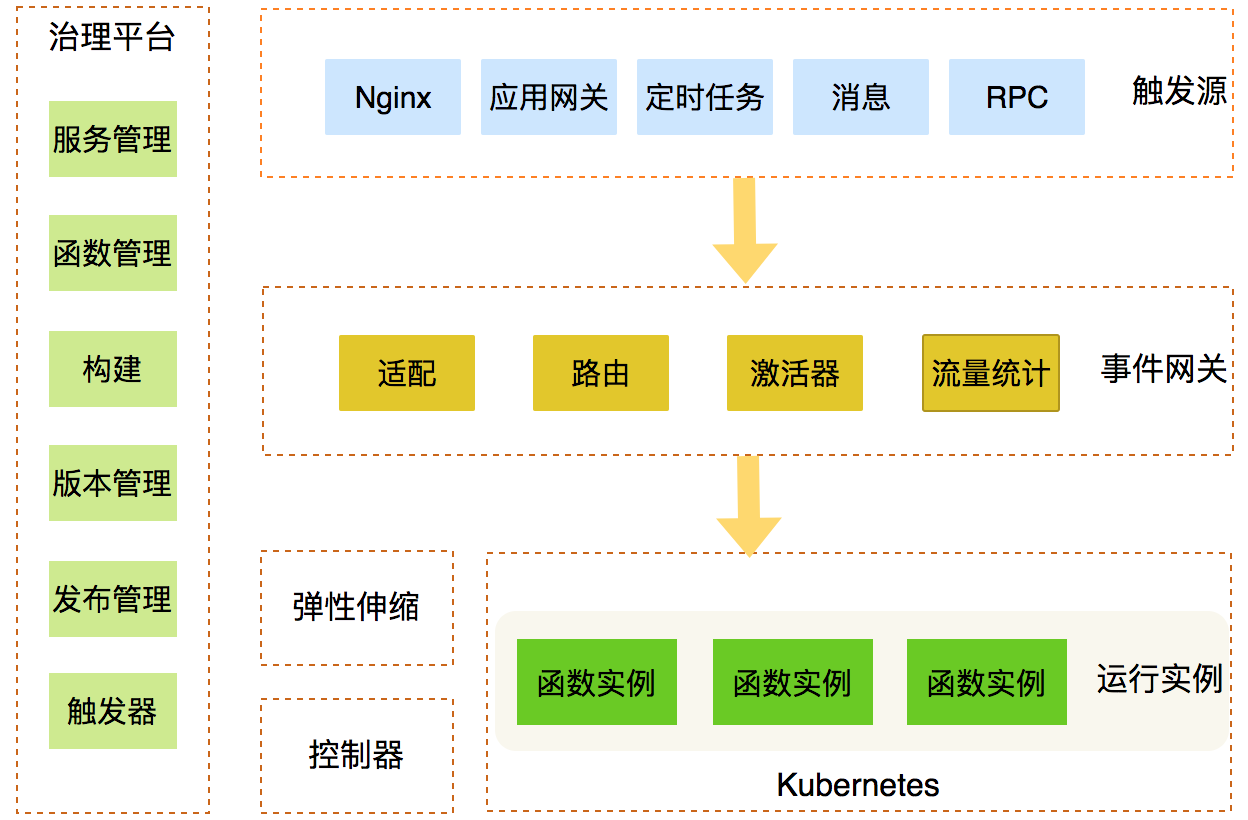
\includegraphics[width=\linewidth]{images/nest_arch.png}
    \caption{美团Nest架构图\cite{meituan_serverless_nest}}
    \label{nest_arch}
\end{figure}

\subsection{AWS Lambda的整体架构}
AWS Lambda平台使用类似微服务的架构,
划分了不同的子系统,
每个子系统负责不同的职责,
其架构如\cref{lambda_services}所示。

\begin{figure}[ht!]
    \centering
    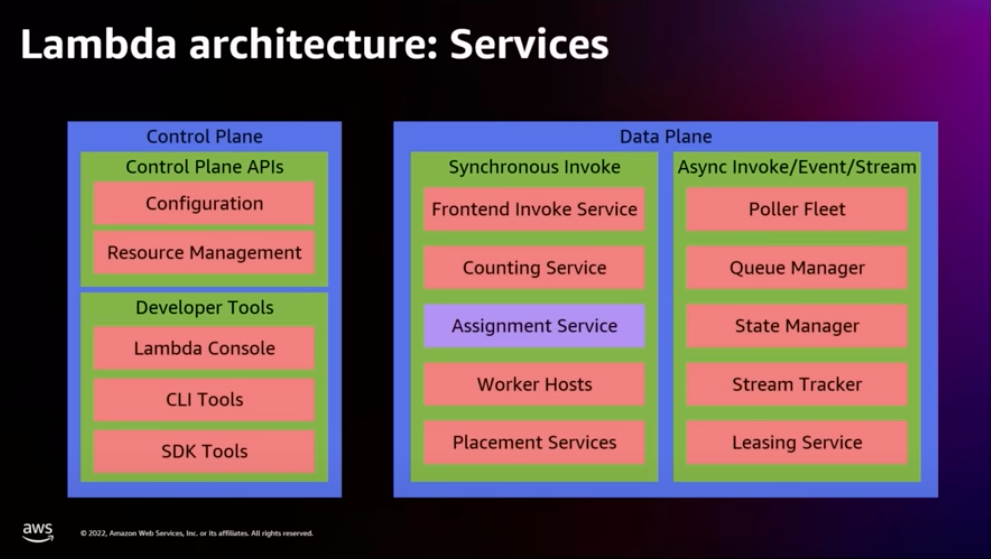
\includegraphics[width=\linewidth]{images/lambda_services.png}
    \caption{AWS Lambda的整体服务划分\cite{aws_lambda_2022}}
    \label{lambda_services}
\end{figure}

Lambda分别使用不同的服务来支持同步异步调用。
同步调用时,
各个系统间的协作关系如\cref{lambda_sync}所示,
其中:

\begin{itemize}
    \item Frontend Invoke Service作为调用入口
    \item Counting Service负责计费信息追踪,
    每次Lambda调用均会调用此服务,
    同时还有并发控制信息
    \item Assignment Service负责为函数调用执行分配一个工作单元
    \item Placement Service负责维护Worker的状态,
    提供基于时间的租约,供Assignment Service获取可用节点信息
    \item Worker 是最终负责执行计算的单元
\end{itemize}


\begin{figure}[ht!]
    \centering
    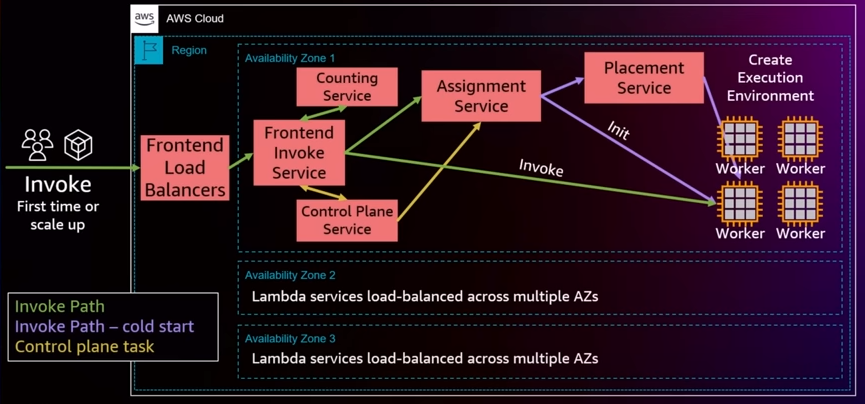
\includegraphics[width=\linewidth]{images/lambda_sync.png}
    \caption{AWS Lambda中的同步调用\cite{aws_lambda_2022}}
    \label{lambda_sync}
\end{figure}

而执行异步任务时,
会首先将其缓存到队列中,
并由Poller负责消费队列中的事件,
然后转化为同步调用,
其过程如\cref{lambda_async}所示。

\begin{figure}[ht!]
    \centering
    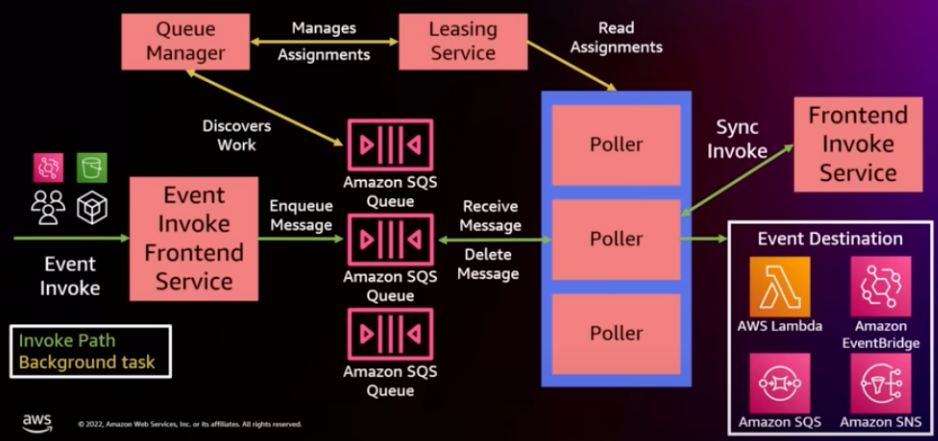
\includegraphics[width=\linewidth]{images/lambda_async.png}
    \caption{AWS Lambda中的异步调用\cite{aws_lambda_2022}}
    \label{lambda_async}
\end{figure}
